\chapter*{Der Campus++}
\addcontentsline{toc}{chapter}{Der Campus++ \hspace*{.1cm} \keys{must read}}

Auch wenn die eine oder der andere sich das vielleicht wünscht, wird sich nicht das gesamte Studium in einem Gebäude abspielen.
Stattdessen gibt es einige wichtige Gebäude, die in deinem Studienalltag eine Rolle spielen werden.

\minisec{HSZ}
Gerade die Grundlagenvorlesungen finden nicht im APB, sondern im Hörsaalzentrum (\emph{HSZ}) statt.
In diesem, im Vergleich zum APB doch sehr eintönigen Gebäude, wirst du viele deiner Vorlesungen erleben und beim Pendeln zwischen APB und HSZ den einen oder anderen Kilometer ansammeln.
Das HSZ umfasst vier Vorlesungssäle, unter Anderem das Audimax, den größten Hörsaal der Universität und das größte Auditorium Sachsens.
Zusätzlich finden sich hier noch einige Seminarräume, in welchen Übungen stattfinden können. Hinter dem \enquote{zentralen Kubus} liegt die schöne Wiese des HSZ\@. Auf ihr kann man nicht nur entspannen. Auch Feste und Messen finden dort regelmäßig statt.
Außerdem steht für den kleinen Hunger dort nicht nur
der Grillcube mit Burgern und Co., sondern auch das Pasta-Mobil mit frischer Pasta.

\minisec{Willersbau}
Der Willersbau~\link{https://navigator.tu-dresden.de/etplan/wil/00} ist das Gebäude der Mathematik an der TU Dresden. Hier finden teilweise deine Matheübungen statt. Der Willersbau ist in direkter Umgebung
des Hörsaalzentrums und des Trefftzbaus, in dem der Mathe-Hörsaal beherbergt ist.

\minisec{Trefftzbau}
Hier~\link{https://navigator.tu-dresden.de/etplan/tre/00} finden i.d.R. Teile deiner Mathevorlesungen statt. Da der Bau gerade saniert wird und Ausnahmen Regeln bestätigen, werden dort auf Grund der Sanierung z.Z. keine Vorlesungen gehalten. Vor dem Trefftzbau befindet sich die Trefftzwiese, die gerade im Sommer wunderbar zum Entspannen nach
einer Vorlesung einlädt.

\begin{figure}[b!]
    \centering
    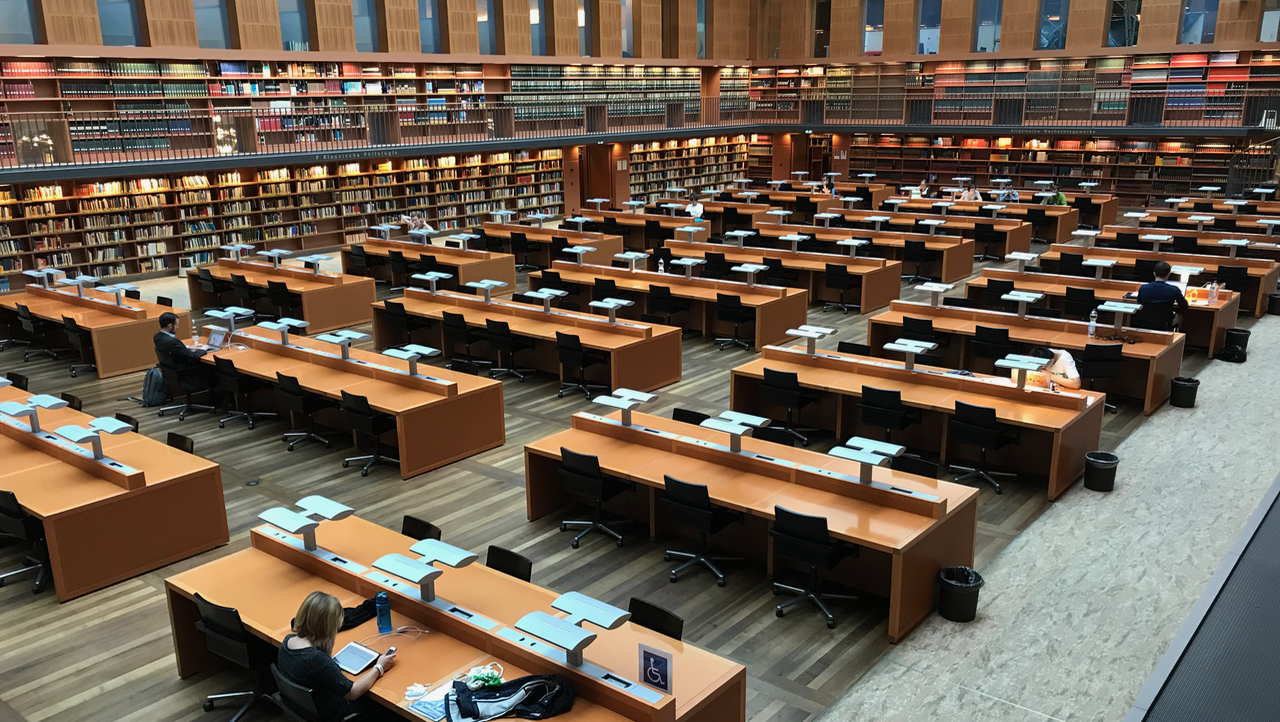
\includegraphics[width=\linewidth]{img/slub-lesesaal}
\end{figure}

\minisec{SLUB}
\label{sec:slub}
Die Sächsische Landesbibliothek – Staats- und Universitätsbibliothek Dresden, kurz \emph{SLUB}~\link{https://slub-dresden.de} ist das, was an anderen Universitäten einfach Bib heißt.
Mit einer Auswahl von über 12 Millionen Bestandseinheiten bestehend aus Büchern, Magazinen, Filmen, etc.\ ist sie eine der größten (Universitäts-) Bibliotheken Deutschlands.
Neben haptisch erlebbarem Lesewerk bietet die SLUB auch eine umfangreiche Auswahl online verfügbarer Ressourcen, die du dir als Studierender kostenfrei herunterladen kannst.
Viele der Bücher, die dir in Grundlagenvorlesungen empfohlen werden, hat die SLUB in großen Stückzahlen vorrätig. Ein Gang in die Lehrbuchabteilung kann dir also viele unnötige Kosten ersparen.
Gegenüber vom Hauptgebäude liegt der DrePunct, eine Zweigstelle der SLUB, in der die meisten Informatik-Fachbücher lagern. Sollte man ein spezifisches Buch suchen, empfiehlt es sich jedoch, vorher auf der Website der
SLUB einmal den Standort des Buches herauszufinden. Dies erspart dir schon einmal den Großteil des Suchweges und zeigt dir an, ob dein Buch der Begierde gerade verfügbar ist.\newline
Doch auch für notorische Nichtleser ist die SLUB aufgrund der vielen Arbeitsplätze ein beliebter Aufenthaltsort.
Willst du mit anderen gemeinsam lernen, gibt es dafür einen weiträumigen Eingangsbereich mit Gruppentischen.
Darüber hinaus können private Gruppenräume reserviert werden. Möchtest du lieber alleine lernen, gibt es natürlich auch genug ruhige Plätze für dich in der SLUB\@. Die ruhigsten Arbeitsplätze findest du im zentralen Lesesaal
im zweiten Untergeschoss, welcher auch im Bild unten zu betrachten ist. Ein schönes Café, in dem per Mensakarte bezahlt werden kann, rundet das Ganze ab.

\newpage
\minisec{Seminargebäude}
Im Seminargebäude, an der besonders schönen Fassade erkennbar, finden die Sprachkurse des LSK statt.
Für alle, die über einen einfachen Sprachkurs hinausgehen wollen, werden zusätzlich Seminare zur Kultur und Politik ausgewählter Länder und Regionen angeboten.
Weitere Informationen findest du auf der Website des LSK~\link{https://tu-dresden.de/gsw/slk/lsk}.
Das Gebäude steht direkt neben der SLUB, zu Fuß ca.\ 20 Minuten vom APB entfernt.

\minisec{Mensen}
Wer sein Studium nicht mit Pizzabestellungen bestreiten will, muss das zum Glück auch nicht, denn das Studierendenwerk betreibt ein Netz aus 18 Mensen.
Egal in welchem Gebäude der Universität du dich befindest, in der Nähe wird eine Mensa oder zumindest ein Café zu finden sein.
Das Tagesangebot aller Mensen ist auf der Seite des Studierendenwerks~\link{https://www.studentenwerk-dresden.de/mensen/speiseplan/} zu finden.

Die Größte der Mensen, die Alte Mensa, befindet sich glücklicherweise direkt zwischen Fakultät und HSZ\@.
Hier findest du eine Vielzahl an täglich wechselnden Hauptgerichten, Salaten und Nachspeisen.
Für Freunde des späten Frühstücks oder Studierende mit gestörtem Schlafrhythmus findet sich in der Alten Mensa zwischen Montag und Donnerstag bis 19 Uhr ein warmes Abendangebot.
Die Auswahl ist jedoch nach 15 Uhr zunehmend eingeschränkter.
Da die Mensa zu Stoßzeiten der Fülle an Menschen kaum standhalten kann, bieten sich Essenszeiten an, die \emph{nicht} direkt nach Ende einer Doppelstunde beginnen.

Sollte dir das Angebot der Alten Mensa nicht zusagen, kannst du den Fußweg von 10 Minuten zum Zeltschlösschen gern in Kauf nehmen. Das Zeltschlösschen ist eine klassische Mensa, die der Alten Mensa in so ziemlich allen Punkten unterlegen ist.

In fünf Minuten kannst du ebenfalls die Bio-Mensa U-Boot erreichen. Der Name ist hier Programm und die in dieser Mensa verwendeten Zutaten sind aus biologischer und lokaler Erzeugung.
Das in der Mensa U-Boot verwendete Fleisch kommt direkt aus dem Westen Dresdens, was den Preis der Mahlzeiten allerdings nicht unerheblich erhöht.
Die Preise der fleischlosen Alternativen sollten sich jedoch nicht sonderlich von denen anderer Mensen unterscheiden.

Auch am Wochenende kannst du dem Kochen entkommen, denn die Mensa Siedepunkt hat auch an Samstagen und Sonntagen geöffnet.
Gerade nach einer produktiven Lerneinheit in der SLUB ist diese ganz bequem mit einem einfachen Wechsel der Straßenseite zu erreichen.

\paragraph{FSR Geheimtipp:}
Ohne Zweifel die beliebteste Mensa auf dem Campus, schenkt man den Aussagen Dresdner FSRlingen glauben, ist Firat.
Es handelt sich hierbei um einen unabhängigen Dönerladen, doch durch den effizienten Umgang mit überdurchschnittlich hohem studentischen Andrang wird er gern auch scherzhaft als Mensa bezeichnet.
Das Dönerhaus liegt knapp 10 Minuten Fußweg vom APB entfernt und lockt mit guter Qualität, gemütlichem Ambiente und einer vergleichsweise großen Auswahl an Gerichten.

\minisec{Studentenklub Count Down}

\begin{wrapfigure}{l}{3cm}%
  \vspace{-.5cm}
  
\includegraphics[width=\linewidth]{img/countdown}
  \vspace{-1cm}
\end{wrapfigure}

Dresden gilt als inoffizielle Hauptstadt der Studentenklubs, immerhin gibt es hier 15 Stück.
Auch der Studentenklub IZ e.V. betreibt in den Tiefen des Wohnheims Güntzstraße 22 einen kleinen Studentenklub, das Count~Down.
IZ steht dabei für Informatikzentrum und tatsächlich ist dies der letzte Rest der Informatikfakultät in der Johannstadt, wo sie bis in die Mitte der 2000er ihre Heimat hatte.

Neben einer großen Auswahl der besten Biere und der leckersten Mate zu studentischen Preisen bietet das Count~Down eine breite Veranstaltungspalette. Spieleabende, verschiedene Metalpartys, der gemeinsame Erasmus-Länderabend mit der ESN-Initiative der TU-Dresden sowie Werwolf- und Cocktailabende gehören zum regelmäßigen Repertoire.
Weitere Informationen findest du unter~\link{https://www.countdown-dresden.de/}.

Natürlich solltest du auch mal bei den anderen Studentenclubs vorbeischauen~\link{https://vdsc.de/}.

Allgemein wird der Betrieb der Studentenclubs durch ehrenamtliches Engagement sichergestellt, daher sind sie immer auf der Suche nach Nachwuchs und frischen Ideen. Melde dich einfach bei deinem Lieblingsclub, wenn du dir vorstellen kannst, auch einmal hinter der Bar zu stehen oder andere Aufgaben zu übernehmen.

\begin{awesomeblock}[ese_bg_color]{2pt}{\faCalendar*[regular]}{ese_bg_color}
    \textbf{Öffnungszeiten}

    Montags: 19 bis 0 Uhr

    Dienstags: 20 bis 1 Uhr

    Mittwochs: 19 bis 0 Uhr

    sowie ausgewählte Samstage
\end{awesomeblock}
